
%%%
% Things that happened after the experiments
%%%

\subsection{Round 1}

%%%
% Discussion of Round 1:
%	1. graphs to show how strategies were learned
%		4-5 frames to get a flip-book/transition to see things go on 1 strategy
%		2-3 different final strategy pngs
%	2. Performance:
%		worse than random agent in tournament play
%%%

%%%
Round 1 consisted of 32 agents with randomly allocated starting weights
paired off against each other.
%
These two agents played one million games against each other,
each starting with a random score,
learning and reinforcing their weight vectors after each game.
%%%

\subsubsection{Learning Process}

%%%
% Discuss flipbook figure
%%%

%%%
The results of the first round's training on a sample agent can be seen
in Figure~\ref{fig_r1-flip}.
%
Each individual square within the image represents the strength of a single
strategy,
in this case \handmaxavg,
where white means completely absent and black means completely dominant.
%
Each image was taken at an intermediate stage to capture and show transitions.
%%%

%%%
There are two things to note from these results.
%
The first is the stark contrast in colors in the majority of the image.
%
The other is the area in which these stark contrasts are present.
%%%

%%%
In the starting phase,
all weights are randomly assigned and relatively uniform with only slight
variances,
hence the blurry dull gray appearance.
%
As time progresses,
the image becomes crisper and filled with more contrast.
%
This indicates not only stronger preference for the strategy at the given
point,
but an almost all-or-nothing attitude towards adhering to a single strategy.
%
This means there is little to no nuance to which cards are chosen
and there is little to no chance for other strategies to collectively overrule 
or veto the major strategy.
%%%

%%%
Also of note is where the previously mentioned stark contrast is present and
where it is absent.
%
Since only those states which have been visited can have their weights
influenced,
the remainder will continue to stay untouched.
%
As can be seen in the top-right and bottom-left corners,
representing extremely unlikely scores to reach in which one player has
achieved a rather large lead while only allowing a few points,
contain only the dull gray of the initial weights.
%
This is because even with a potential spread of 60 points when initialized,
these outlandish scores are outside the realm of potential visitation.
%
Therefore, they have not been a part of any game,
so they cannot have their weights adjusted.
%%%

% Figure for the flipbook of strategies over time

\begin{figure}
\center

	\begin{subfigure}[t]{0.3\textwidth}
	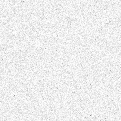
\includegraphics[width=\textwidth]{images/findings/round1/flipbook_a.png}
	\caption{Starting Weights}
	\end{subfigure}
	~
	\begin{subfigure}[t]{0.3\textwidth}
	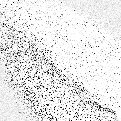
\includegraphics[width=\textwidth]{images/findings/round1/flipbook_b.png}
	\caption{After 200,000 games played}
	\end{subfigure}
	~
	\begin{subfigure}[t]{0.3\textwidth}
	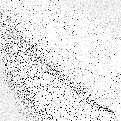
\includegraphics[width=\textwidth]{images/findings/round1/flipbook_c.png}
	\caption{After 400,000 games played}
	\end{subfigure}

	\begin{subfigure}[t]{0.3\textwidth}
	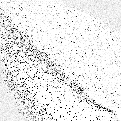
\includegraphics[width=\textwidth]{images/findings/round1/flipbook_d.png}
	\caption{After 600,000 games played}
	\end{subfigure}
	~
	\begin{subfigure}[t]{0.3\textwidth}
	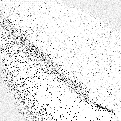
\includegraphics[width=\textwidth]{images/findings/round1/flipbook_e.png}
	\caption{After 800,000 games played}
	\end{subfigure}
	~
	\begin{subfigure}[t]{0.3\textwidth}
	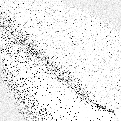
\includegraphics[width=\textwidth]{images/findings/round1/flipbook_f.png}
	\caption{Final Weights}
	\end{subfigure}

\caption{%
	Training weights representation for Agent 0's \handmaxavg\
	strategy when the agent is the dealer
	over the course of the one million games of Round 1.
	In these images, the y-axis represents the player's own score,
	the x-axis the opponent's score,
	with the origin starting at the top-left of the image.
	% N.B. This is correct of generated images from the python code
	%	as of 2018-03-08 19:12.
	% no later modifications will be made from the python code directly to
	% save myself the headache. maybe this will be converted later to be
	% more easily human understood
	% Rotate 90 deg counter-clockwise will make x=my_score, y=opp_score
}
% TODO: figure out axes
% TODO: change these images to hand_max_min: much starker contrast
\label{fig_r1-flip}
\end{figure}


\begin{figure}
\center

	\begin{subfigure}[t]{0.22\textwidth}
		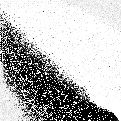
\includegraphics[width=\textwidth]{images/findings/round1/strategies_handmaxmin.png}
		\caption{\handmaxmin}
	\end{subfigure}
	~
	\begin{subfigure}[t]{0.22\textwidth}
		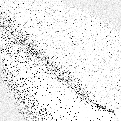
\includegraphics[width=\textwidth]{images/findings/round1/strategies_handmaxavg.png}
		\caption{\handmaxavg}
	\end{subfigure}
	~
	\begin{subfigure}[t]{0.22\textwidth}
		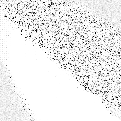
\includegraphics[width=\textwidth]{images/findings/round1/strategies_handmaxmed.png}
		\caption{\handmaxmed}
	\end{subfigure}
	~
	\begin{subfigure}[t]{0.22\textwidth}
		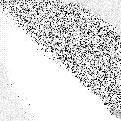
\includegraphics[width=\textwidth]{images/findings/round1/strategies_handmaxposs.png}
		\caption{\handmaxposs}
	\end{subfigure}

	\begin{subfigure}[t]{0.22\textwidth}
		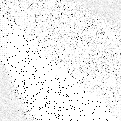
\includegraphics[width=\textwidth]{images/findings/round1/strategies_cribminavg.png}
		\caption{\cribminavg}
	\end{subfigure}
	~
	\begin{subfigure}[t]{0.22\textwidth}
		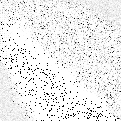
\includegraphics[width=\textwidth]{images/findings/round1/strategies_peggingmaxavggained.png}
		\caption{\peggingmaxavggained}
	\end{subfigure}
	~
	\begin{subfigure}[t]{0.22\textwidth}
		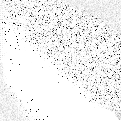
\includegraphics[width=\textwidth]{images/findings/round1/strategies_peggingmaxmedgained.png}
		\caption{\peggingmaxmedgained}
	\end{subfigure}
	~
	\begin{subfigure}[t]{0.22\textwidth}
		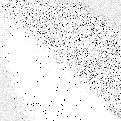
\includegraphics[width=\textwidth]{images/findings/round1/strategies_peggingminavggiven.png}
		\caption{\peggingminavggiven}
	\end{subfigure}

\caption{
	All final strategy strengths for Agent 0
	when playing as the dealer
	after training for one million games during Round 1.
}
% TODO: figure out axes
\label{fig_r1-strats}
\end{figure}

\begin{figure}
\center

	\begin{subfigure}[t]{0.22\textwidth}
		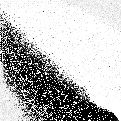
\includegraphics[width=\textwidth]{images/findings/round1/strategies_handmaxmin_pone.png}
		\caption{\handmaxmin}
	\end{subfigure}
	~
	\begin{subfigure}[t]{0.22\textwidth}
		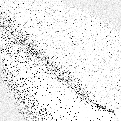
\includegraphics[width=\textwidth]{images/findings/round1/strategies_handmaxavg_pone.png}
		\caption{\handmaxavg}
	\end{subfigure}
~
	\begin{subfigure}[t]{0.22\textwidth}
		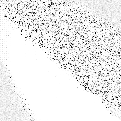
\includegraphics[width=\textwidth]{images/findings/round1/strategies_handmaxmed_pone.png}
		\caption{\handmaxmed}
	\end{subfigure}
	~
	\begin{subfigure}[t]{0.22\textwidth}
		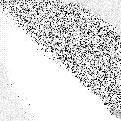
\includegraphics[width=\textwidth]{images/findings/round1/strategies_handmaxposs_pone.png}
		\caption{\handmaxposs}
	\end{subfigure}

	\begin{subfigure}[t]{0.22\textwidth}
		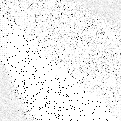
\includegraphics[width=\textwidth]{images/findings/round1/strategies_cribminavg_pone.png}
		\caption{\cribminavg}
	\end{subfigure}
	~
	\begin{subfigure}[t]{0.22\textwidth}
		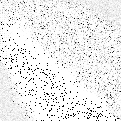
\includegraphics[width=\textwidth]{images/findings/round1/strategies_peggingmaxavggained_pone.png}
		\caption{\peggingmaxavggained}
	\end{subfigure}
~
	\begin{subfigure}[t]{0.22\textwidth}
		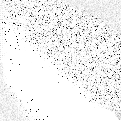
\includegraphics[width=\textwidth]{images/findings/round1/strategies_peggingmaxmedgained_pone.png}
		\caption{\peggingmaxmedgained}
	\end{subfigure}
	~
	\begin{subfigure}[t]{0.22\textwidth}
		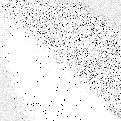
\includegraphics[width=\textwidth]{images/findings/round1/strategies_peggingminavggiven_pone.png}
		\caption{\peggingminavggiven}
	\end{subfigure}

\caption{
	All final strategy strengths for an agent
	when playing as the pone
	after training for one million games during Round 1.
}
\label{fig_r1-strats-pone}
\end{figure}



\subsubsection{Learning Results}

%%%
% Discuss Strategies Figure
%%%

%%%
Despite the all-or-nothing nature of how a single strategy is potentially
learned,
it is still worth noting that the agent did in fact learn to play different
strategies at different times.
%
As can be seen in Figure~\ref{fig_r1-strats},
the strengths of each strategy's weight do vary across score-locations.
%
For instance, when in the lead by
roughly two to twenty five points,
the agent will prefer to choose the hand with the most guaranteed
points in its own hand
by following \handmaxmin.
%
However, when the game is either extremely close
or when the agent is well in the lead,
the agent will take a slight gamble and play for expected points.
%
Occasionally, the agent will also attempt to pay attention to the points
gained through the play phase of a round by playing a combination that pegs
well.
%
Ironically,
the agent may play against its own best wishes by minimizing the average return
of the crib.
%
This is speculated to be a result of alignment of the results between
\cribminavg\ and more reasonable \handmaxmin\
or \handmaxavg.
%%%

%%%
Of further interest is how little the agent knows how to handle a losing
position.
%
As can be seen by looking in the upper-right half of each strategy's
individual graph,
of the explored losing states,
there is little consensus or pattern as to which strategy should dominate.
%
It is possible that agents which end up in these positions lose more often than
they win.
%
If this is the case,
the resulting punishment will decrease the top two or three strategies that were
most responsible for the hand choice at that state,
effectively increasing all others.
%
This in turn would likely later lead to a cycle in which different strategies
are cyclically placed in a role of strongest weight,
generating the fuzz seen now.
%%%


%%%
% TODO: Similarity/differences between dealer and pone
%%%

%%%
By comparing the pone's strategy graphs to those of the dealer's,
a few patterns emerge.
%
At first glance,
the graphs look highly similar and as if splitting up the search space into two
merely increased the complexity of finding a solution without payoff.
%
For instance,
the majority of the winning positions favor the \handmaxmin\ strategy with
a ``border'' of \handmaxavg\ being used in positions where riskier decisions
are needed or can be afforded.
%
Additionally, the losing positions offer no definitive answers and seem to be a
jumbled mess of suggestions,
the only major suggestion being to play more riskily to regain the lead.
%%%

%%%
However, upon closer inspection,
with a side-by-side\textemdash or perhaps even overlaying\textemdash comparison,
there are subtle differences that can be found.
%
The most major of these differences is that all patterns are shifted lower and
more to the left when the agent is the dealer,
correlating with scores which are more advantageous to the player
%
This means that the agent is more ``comfortable'' when it has a slightly larger
lead as the dealer than it necessarily needs as the pone.
%
It also means that the unexplored state area as the pone is larger in the area
where it is further ahead.
%
% TODO: continue this thought
%%%


%%%
% Bump/sinusoidal wave in final game stages
%		+ how they differ b/w dealer and pone
%%%

%%%
Perhaps the most interesting difference is the traceable shape of the weights
during the final scores of a close game.
%
Although difficult to discern in all but the \handmaxmin\ and \handmaxavg\ 
strategies,
the final weights trace a sinusoidal curve shape along the diagonal
for approximately the last twenty points of the game.
%
Additionally,
these waves are opposing in nature.
%
This presents the fascinating conclusion that the agent is learning
that different states or checkpoints are preferred as the player when
the dealer and when the pone.
%
Not only is this fascinating since the agent is learning a state-value function
indirectly,
but in the game of cribbage,
there exist different \textit{checkpoints} in which the player aims to get
himself by the end of a round to be in favorable position for the next.
%
Here we see evidence that the agent is learning these checkpoints throughout its
play.
%%%


\subsubsection{Performance}

%%%
% discuss how it performed worse than random (got stonked)
While it is
aggravating that the agent learns to over-trust a single strategy,
it is simultaneously reassuring that general trends in play are detected.
%
However, perhaps the only metric which matters from a learning perspective is
the agent's performance.
%
In this area, the learned agents failed miserably.
%
The winning agent between the two learners was pitted against
an agent using randomly allocated starting weights
where both agents would only strictly follow the policy generated
without exploration.
%
As can be seen in Table~\ref{tab_r1-randtourny},
the learned agent lost easily to the randomly-weighted agent:
with the exception of a spectacular loss in Game 3,
all other games were close losses if not wins.
%
This is speculated to be a result of the previously mentioned over-aggressive
learning pattern and its all-or-nothing end result.
%
Since the agent aligns so intensely to a single strategy,
it is not able to overcome a local optimum
and has essentially been overfit to the scenario.
%
Another potential reason for the losses could be the lack of knowledge of how to
handle losing situations.
%
As previously discussed,
in the event of a loss,
most strategies will effectively be increased except those most responsible,
contributing to a system of cycling weights.
%
Furthermore, it is also likely that an agent which finds itself in a losing
position does not end up recovering and winning the game,
meaning that
the agent effectively learns that it is mostly by chance that it will recover.
%%%

% Table to represent the tournament information

\begin{table}
\center
\begin{tabular}{|r|c|c|}
	\hline
	\textbf{Game} & \textbf{Random} & \textbf{Agent 1}\\\hline

	1 & 104 & 121 \\\hline
	2 & 121 & 114 \\\hline
	3 &  75 & 121 \\\hline
	4 & 121 & 118 \\\hline
	5 & 111 & 121 \\\hline
	6 & 121 &  99 \\\hline
	7 & 121 &  87 \\\hline
	8 & 110 & 121 \\\hline
	9 & 121 &  64 \\\hline

\end{tabular}
~
\begin{tabular}{|r|c|c|c|}
	\hline
	\textbf{Agent} & \textbf{Score} & \textbf{Point Spread} & \textbf{Wins}
	\\\hline
	Random & 12 & +39 & 5
	\\\hline
	Agent 1 & 9 & \textemdash & 4
	\\\hline
\end{tabular}

\label{tab:r1-randtourny}

\caption{
	Results of a nine-game tournament played between
	a randomly-weighted agent
	and
	Agent 1 after learning for one million games.
}

\end{table}


%%%
% discussion of playing an agent against a previous version of itself
%%%

%%%
In order to more accurately diagnose if an overfitting situation was occurring,
a winning agent was played against its own previous checkpoints.
%
A sample set of scores can be found in Table~\ref{tab_r1-selftourny}.
%
The point spreads from twenty separate 100-game tournaments
are depicted in Figure~\ref{fig_r1-spreads_a}.
%
While point spreads are from total points pegged to the board
not gained from wins
and therefore not a direct indicator of performance in tournament play,
it is useful for determining general performance.
%
As can be seen, there is no discernible correlation or pattern between
epoch checkpoint and performance.
%
This indicates that,
despite a policy being learned,
quite a lot is still left to chance of the cards dealt.
%
This has the potential to be exacerbated even further when policies are nearly
deterministic and non-adaptive in their weight assignments.
%
Additionally,
a random agent was played against its future iterations in the same fashion,
with the similar results depicted in Table~\ref{tab_r1-spreads_b}.
%%%


% Table of results for an agent against itself

 % TODO: fill in with actual data

\begin{table}
\center

\begin{tabular}{|r|c|c|c|}
	\hline
	\textbf{Epochs} & \textbf{Score} & \textbf{Spread} & \textbf{Wins}
	\\\hline
	0 & 126 & +523 & 59
	\\\hline
	1MM & 86 & \textemdash & 41
	\\\hline
\end{tabular}
~
\begin{tabular}{|r|c|c|c|}
	\hline
	\textbf{Epochs} & \textbf{Score} & \textbf{Spread} & \textbf{Wins}
	\\\hline
	100K & 122 & +200 & 55
	\\\hline
	1MM & 104 & \textemdash & 45
	\\\hline
\end{tabular}

\begin{tabular}{|r|c|c|c|}
	\hline
	\textbf{Epochs} & \textbf{Score} & \textbf{Spread} & \textbf{Wins}
	\\\hline
	200K & 108 & -27 & 47
	\\\hline
	1MM & 118 & \textemdash & 53
	\\\hline
\end{tabular}
~
\begin{tabular}{|r|c|c|c|}
	\hline
	\textbf{Epochs} & \textbf{Score} & \textbf{Spread} & \textbf{Wins}
	\\\hline
	300K & 105 & -180 & 48
	\\\hline
	1MM & 116 & \textemdash & 52
	\\\hline
\end{tabular}

\begin{tabular}{|r|c|c|c|}
	\hline
	\textbf{Epochs} & \textbf{Score} & \textbf{Spread} & \textbf{Wins}
	\\\hline
	400K & 87 & -510 & 41
	\\\hline
	1MM & 133 & \textemdash & 59
	\\\hline
\end{tabular}
~
\begin{tabular}{|r|c|c|c|}
	\hline
	\textbf{Epochs} & \textbf{Score} & \textbf{Spread} & \textbf{Wins}
	\\\hline
	500K & 97 & -386 & 43
	\\\hline
	1MM & 129 & \textemdash & 57
	\\\hline
\end{tabular}

\begin{tabular}{|r|c|c|c|}
	\hline
	\textbf{Epochs} & \textbf{Score} & \textbf{Spread} & \textbf{Wins}
	\\\hline
	600K & 117 & 370 & 52
	\\\hline
	1MM & 98 & \textemdash & 48
	\\\hline
\end{tabular}
~
\begin{tabular}{|r|c|c|c|}
	\hline
	\textbf{Epochs} & \textbf{Score} & \textbf{Spread} & \textbf{Wins}
	\\\hline
	700K & 107 & -174 & 48
	\\\hline
	1MM & 115 & \textemdash & 52
	\\\hline
\end{tabular}

\begin{tabular}{|r|c|c|c|}
	\hline
	\textbf{Epochs} & \textbf{Score} & \textbf{Spread} & \textbf{Wins}
	\\\hline
	800K & 124 & 239 & 56
	\\\hline
	1MM & 96 & \textemdash & 44
	\\\hline
\end{tabular}
~
\begin{tabular}{|r|c|c|c|}
	\hline
	\textbf{Epochs} & \textbf{Score} & \textbf{Spread} & \textbf{Wins}
	\\\hline
	900K & 111 & -82 & 51
	\\\hline
	1MM & 111 & \textemdash & 49
	\\\hline
\end{tabular}


%%%%%%%%
%
%\begin{tabular}{|r|c|c|c|}
%	\hline
%	\textbf{Epochs} & \textbf{Score} & \textbf{Spread} & \textbf{Wins}
%	\\\hline
%	100K & 104 & -108 & 50
%	\\\hline
%	1MM & 111 & \textemdash & 50
%	\\\hline
%\end{tabular}
%~
%\begin{tabular}{|r|c|c|c|}
%	\hline
%	\textbf{Epochs} & \textbf{Score} & \textbf{Spread} & \textbf{Wins}
%	\\\hline
%	250K & 104 & -268 & 47
%	\\\hline
%	1MM & 121 & \textemdash & 53
%	\\\hline
%\end{tabular}
%
%~
%
%\begin{tabular}{|r|c|c|c|}
%	\hline
%	\textbf{Epochs} & \textbf{Score} & \textbf{Spread} & \textbf{Wins}
%	\\\hline
%	500K & 104 & -116 & 49
%	\\\hline
%	1MM & 109 & \textemdash & 51
%	\\\hline
%\end{tabular}
%~
%\begin{tabular}{|r|c|c|c|}
%	\hline
%	\textbf{Epochs} & \textbf{Score} & \textbf{Spread} & \textbf{Wins}
%	\\\hline
%	750K & 113 & +33 & 53
%	\\\hline
%	1MM & 104 & \textemdash & 47
%	\\\hline
%\end{tabular}

\label{tab:r1-selftourny}

\caption{
	Results of multiple 100-game tournaments played between
	agents using various epoch checkpoints from the training
	and the final agent from the round.
	The weights used here are from Agent 1.
}

\end{table}


% Point spreads for two runs of blah

\begin{figure}
\center

\begin{subfigure}[b]{0.8\textwidth}
	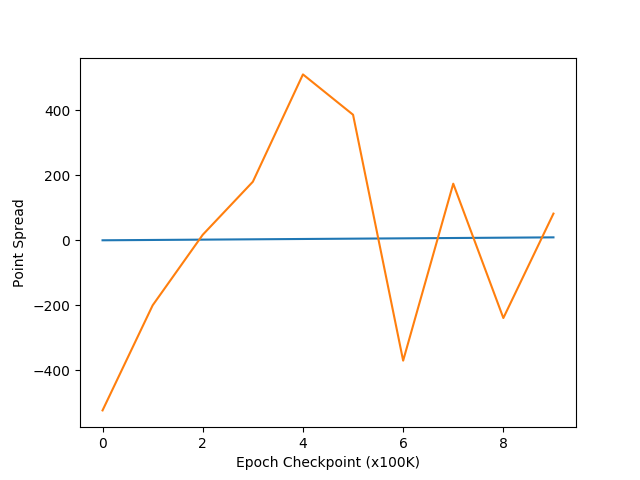
\includegraphics[width=\linewidth]{images/findings/round1/spread1.png}
	\label{fig_r1-spreads_a}
	\caption{}
\end{subfigure}

\begin{subfigure}[b]{0.8\textwidth}
	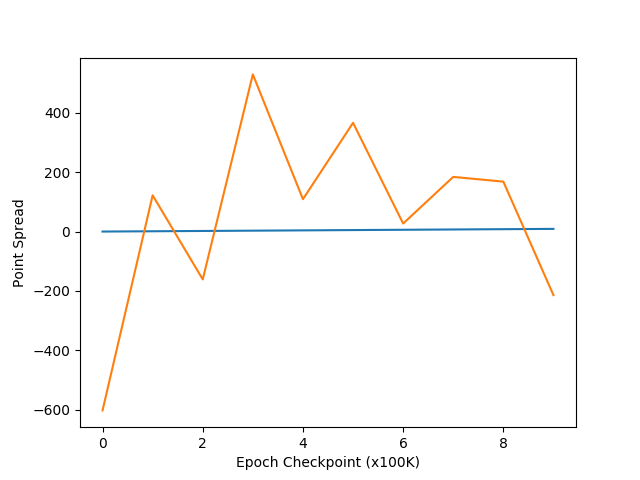
\includegraphics[width=\linewidth]{images/findings/round1/spread2.png}
	\label{fig_r1-spreads_b}
	\caption{}
\end{subfigure}

\caption{
	Point spreads across two 100-game tournaments pitting a winning
	agent against its checkpoints.
	Here, a positive point spread indicates that the fully-trained agent has
	accumulated more points than its opponent,
	an agent created from a checkpoint generated after the number of training
	game epochs indicated on the x-axis.
}
\label{fig_r1-spreads}
\end{figure}



\subsubsection{Applications for Round 2}

%%%
% "Lessons Learned" / changes made
%	Learning rate lowered
%	exploration rate constant
%	trained random v learning in order to learn the game
%%%

%%%
% discuss how the meta-parameters were tweaked for round 2
%		and how the tournament structure got wonked
%%%

%%%
As a result of the over-aggressive learning of single strategies,
some learning parameters were altered for Round 2.
%
Since it was estimated to be the primary reason for the learning behavior,
the first parameter tweak made was to decrease the learning rate drastically.
%
The learning rate was decreased to one fifth of what was used in Round 1.
%
The other major parameter alteration was to make the exploration rate a constant
and not dependent upon the variance of the weights.
%
Because of the stipulation on the variance previously explained in the Methods
section,
the most strongly biased weight locations would only allow for exploration
even more rarely than before.
%
Although only producing a decrease from about a 30\% chance to 18\%,
this would still result in a smaller likelihood of exploring in the current 
state,
potentially further cementing of the dominant strategy in its position.
%
Additionally,
it was a complication which upon further thought would not result in much
difference over the course of time
and thus deemed non-beneficial and ultimately unnecessary.
%%%

%%%
% tournament structure
%%%

%%%
In order to see if the heavily biased weights could be tempered down to more
reasonable mixes which could outplay a random agent,
the structure of the tournament was updated.
%
In addition to having the winners of the previous pair of agents square
off against one another,
there was a ``loser's bracket'' created
in which the losers would start over from ground zero.
%
These two ways of playing were intended as a two-pronged approach
in order to see if multiple agents could be trained at the same time
which could outperform random.
%
The ``winners bracket'' would determine if a highly-biased set of agents could
learn nuance
while the ``losers bracket'' would test if it were possible for two constantly
competing agents could ever actually increase performance when both are each
updating their parameters to combat each other.
%%%

%%%
% random v learning
%	two agents paired with two random agents
%	one learns, other stays the same. learns game, not how to outmatch opponent
%%%

%%%
Since the agents were diagnosed with learning how to outplay each other
but not the game,
the next phase would attempt to determine the extent of this tailored learning.
%
In addition to the previously mentioned alterations to the tournament structure,
a new batch of agents would be trained against a static, entirely random agent.
%
Rather than both agents in the game learning and altering their weights after
each game,
only one agent would train its weights.
%
The prevailing logic behind this decision was that if each agent was indirectly
affecting the other,
the environment could be said to be slightly altered.
%
This would in turn mean that the agents are no longer learning the original
problem.
%%%

